\documentclass[12pt,letterpaper]{article}
\usepackage{graphicx,textcomp}
\usepackage{natbib}
\usepackage{setspace}
\usepackage{fullpage}
\usepackage{color}
\usepackage[reqno]{amsmath}
\usepackage{amsthm}
\usepackage{fancyvrb}
\usepackage{amssymb,enumerate}
\usepackage[all]{xy}
\usepackage{endnotes}
\usepackage{lscape}
\newtheorem{com}{Comment}
\usepackage{float}
\usepackage{hyperref}
\newtheorem{lem} {Lemma}
\newtheorem{prop}{Proposition}
\newtheorem{thm}{Theorem}
\newtheorem{defn}{Definition}
\newtheorem{cor}{Corollary}
\newtheorem{obs}{Observation}
\usepackage[compact]{titlesec}
\usepackage{dcolumn}
\usepackage{tikz}
\usetikzlibrary{arrows}
\usepackage{multirow}
\usepackage{xcolor}
\newcolumntype{.}{D{.}{.}{-1}}
\newcolumntype{d}[1]{D{.}{.}{#1}}
\definecolor{light-gray}{gray}{0.65}
\usepackage{url}
\usepackage{listings}
\usepackage{color}

\definecolor{codegreen}{rgb}{0,0.6,0}
\definecolor{codegray}{rgb}{0.5,0.5,0.5}
\definecolor{codepurple}{rgb}{0.58,0,0.82}
\definecolor{backcolour}{rgb}{0.95,0.95,0.92}

\lstdefinestyle{mystyle}{
	backgroundcolor=\color{backcolour},   
	commentstyle=\color{codegreen},
	keywordstyle=\color{magenta},
	numberstyle=\tiny\color{codegray},
	stringstyle=\color{codepurple},
	basicstyle=\footnotesize,
	breakatwhitespace=false,         
	breaklines=true,                 
	captionpos=b,                    
	keepspaces=true,                 
	numbers=left,                    
	numbersep=5pt,                  
	showspaces=false,                
	showstringspaces=false,
	showtabs=false,                  
	tabsize=2
}
\lstset{style=mystyle}
\newcommand{\Sref}[1]{Section~\ref{#1}}
\newtheorem{hyp}{Hypothesis}

\title{Problem Set 1}
\date{Due: February 11, 2024}
\author{Idi . Applied Stats II}


\begin{document}
	\maketitle
	\section*{Instructions}
	\begin{itemize}
	\item Please show your work! You may lose points by simply writing in the answer. If the problem requires you to execute commands in \texttt{R}, please include the code you used to get your answers. Please also include the \texttt{.R} file that contains your code. If you are not sure if work needs to be shown for a particular problem, please ask.
\item Your homework should be submitted electronically on GitHub in \texttt{.pdf} form.
\item This problem set is due before 23:59 on Sunday February 11, 2024. No late assignments will be accepted.
	\end{itemize}

	\vspace{.25cm}
\section*{Question 1} 
\vspace{.25cm}
\noindent The Kolmogorov-Smirnov test uses cumulative distribution statistics test the similarity of the empirical distribution of some observed data and a specified PDF, and serves as a goodness of fit test. The test statistic is created by:

$$D = \max_{i=1:n} \Big\{ \frac{i}{n}  - F_{(i)}, F_{(i)} - \frac{i-1}{n} \Big\}$$

\noindent where $F$ is the theoretical cumulative distribution of the distribution being tested and $F_{(i)}$ is the $i$th ordered value. Intuitively, the statistic takes the largest absolute difference between the two distribution functions across all $x$ values. Large values indicate dissimilarity and the rejection of the hypothesis that the empirical distribution matches the queried theoretical distribution. The p-value is calculated from the Kolmogorov-
Smirnoff CDF:

$$p(D \leq x) \frac{\sqrt {2\pi}}{x} \sum _{k=1}^{\infty }e^{-(2k-1)^{2}\pi ^{2}/(8x^{2})}$$


\noindent which generally requires approximation methods (see \href{https://core.ac.uk/download/pdf/25787785.pdf}{Marsaglia, Tsang, and Wang 2003}). This so-called non-parametric test (this label comes from the fact that the distribution of the test statistic does not depend on the distribution of the data being tested) performs poorly in small samples, but works well in a simulation environment. Write an \texttt{R} function that implements this test where the reference distribution is normal. Using \texttt{R} generate 1,000 Cauchy random variables (\texttt{rcauchy(1000, location = 0, scale = 1)}) and perform the test (remember, use the same seed, something like \texttt{set.seed(123)}, whenever you're generating your own data).\\
	
	
\noindent As a hint, you can create the empirical distribution and theoretical CDF using this code:

\begin{lstlisting}[language=R]
	# create empirical distribution of observed data
	ECDF <- ecdf(data)
	empiricalCDF <- ECDF(data)
	# generate test statistic
	D <- max(abs(empiricalCDF - pnorm(data))) \end{lstlisting}

\vspace{3in}

\subsection{Answer Q1}
\noindent Here but text answer

\begin{Verbatim}
	this is just  a test
	\\\\\\\\
	> result <- ks_test_normal(cauchy_data)
	> head(result) #blabla
	$test_statistic
	[1] 0.1439423
	
	$p_value
	[1] 1.379198e-52
	
	$conclusion
	[1] "Reject Null Hypothesis"
\end{Verbatim}

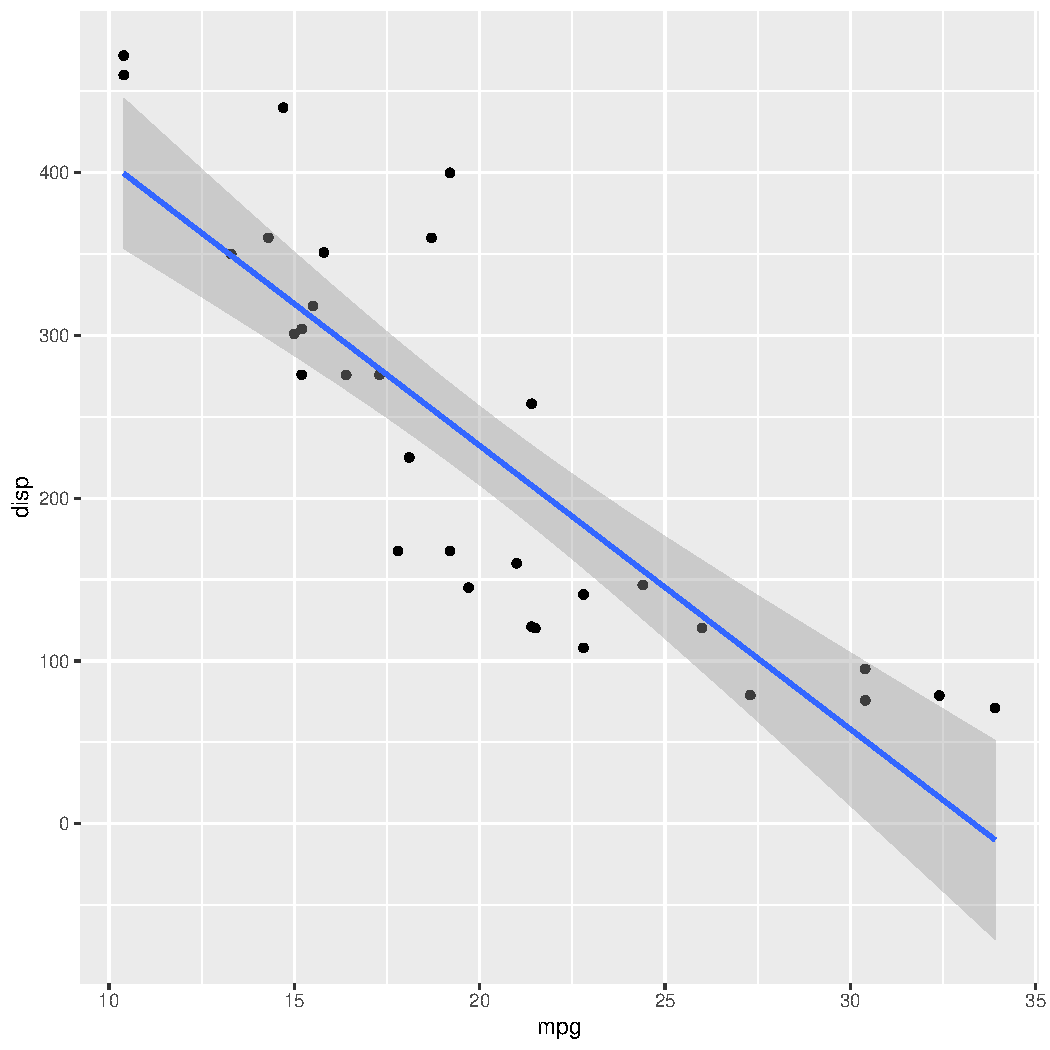
\includegraphics{test.pdf}

\section*{Question 2}
\noindent Estimate an OLS regression in \texttt{R} that uses the Newton-Raphson algorithm (specifically \texttt{BFGS}, which is a quasi-Newton method), and show that you get the equivalent results to using \texttt{lm}. Use the code below to create your data.
\vspace{.5cm}
\lstinputlisting[language=R, firstline=51,lastline=53]{PS1.R} 

\end{document}
